\section{実験}

改造したMiniSatと実装した遺伝アルゴリズムを用いて実際に証明の作成を行なった。
主な実験として
\begin{enumerate}
    \item 遺伝アルゴリズムのパラメータを調整して、短い証明を作りやすくするための実験
    \item 調整を行なった遺伝アルゴリズムがどれぐらいの効果あるかをみる実験
    \item 最先端のソルバーと比べてどれぐらい短い証明が作れているのかをみる実験
\end{enumerate}
の3種類の実験をおこなった。
実験のために用いる問題は、SATソルバの性能を測る大会SAT compの2016年のAgileトラックにおいての問題を使用した。

% 問題の設定
% どういう実験を行なったか

\setcounter{subsection}{-1}

\subsection{事前実験}%1ページ

・1変数介入の実験

・10回の介入をずらしながら実験

\subsection{パラメータ調整}%5ページ

1とりあえず

 ・サイズ5 * 世代20

 ・初期介入回数10

\begin{figure}[h]
    \centering
    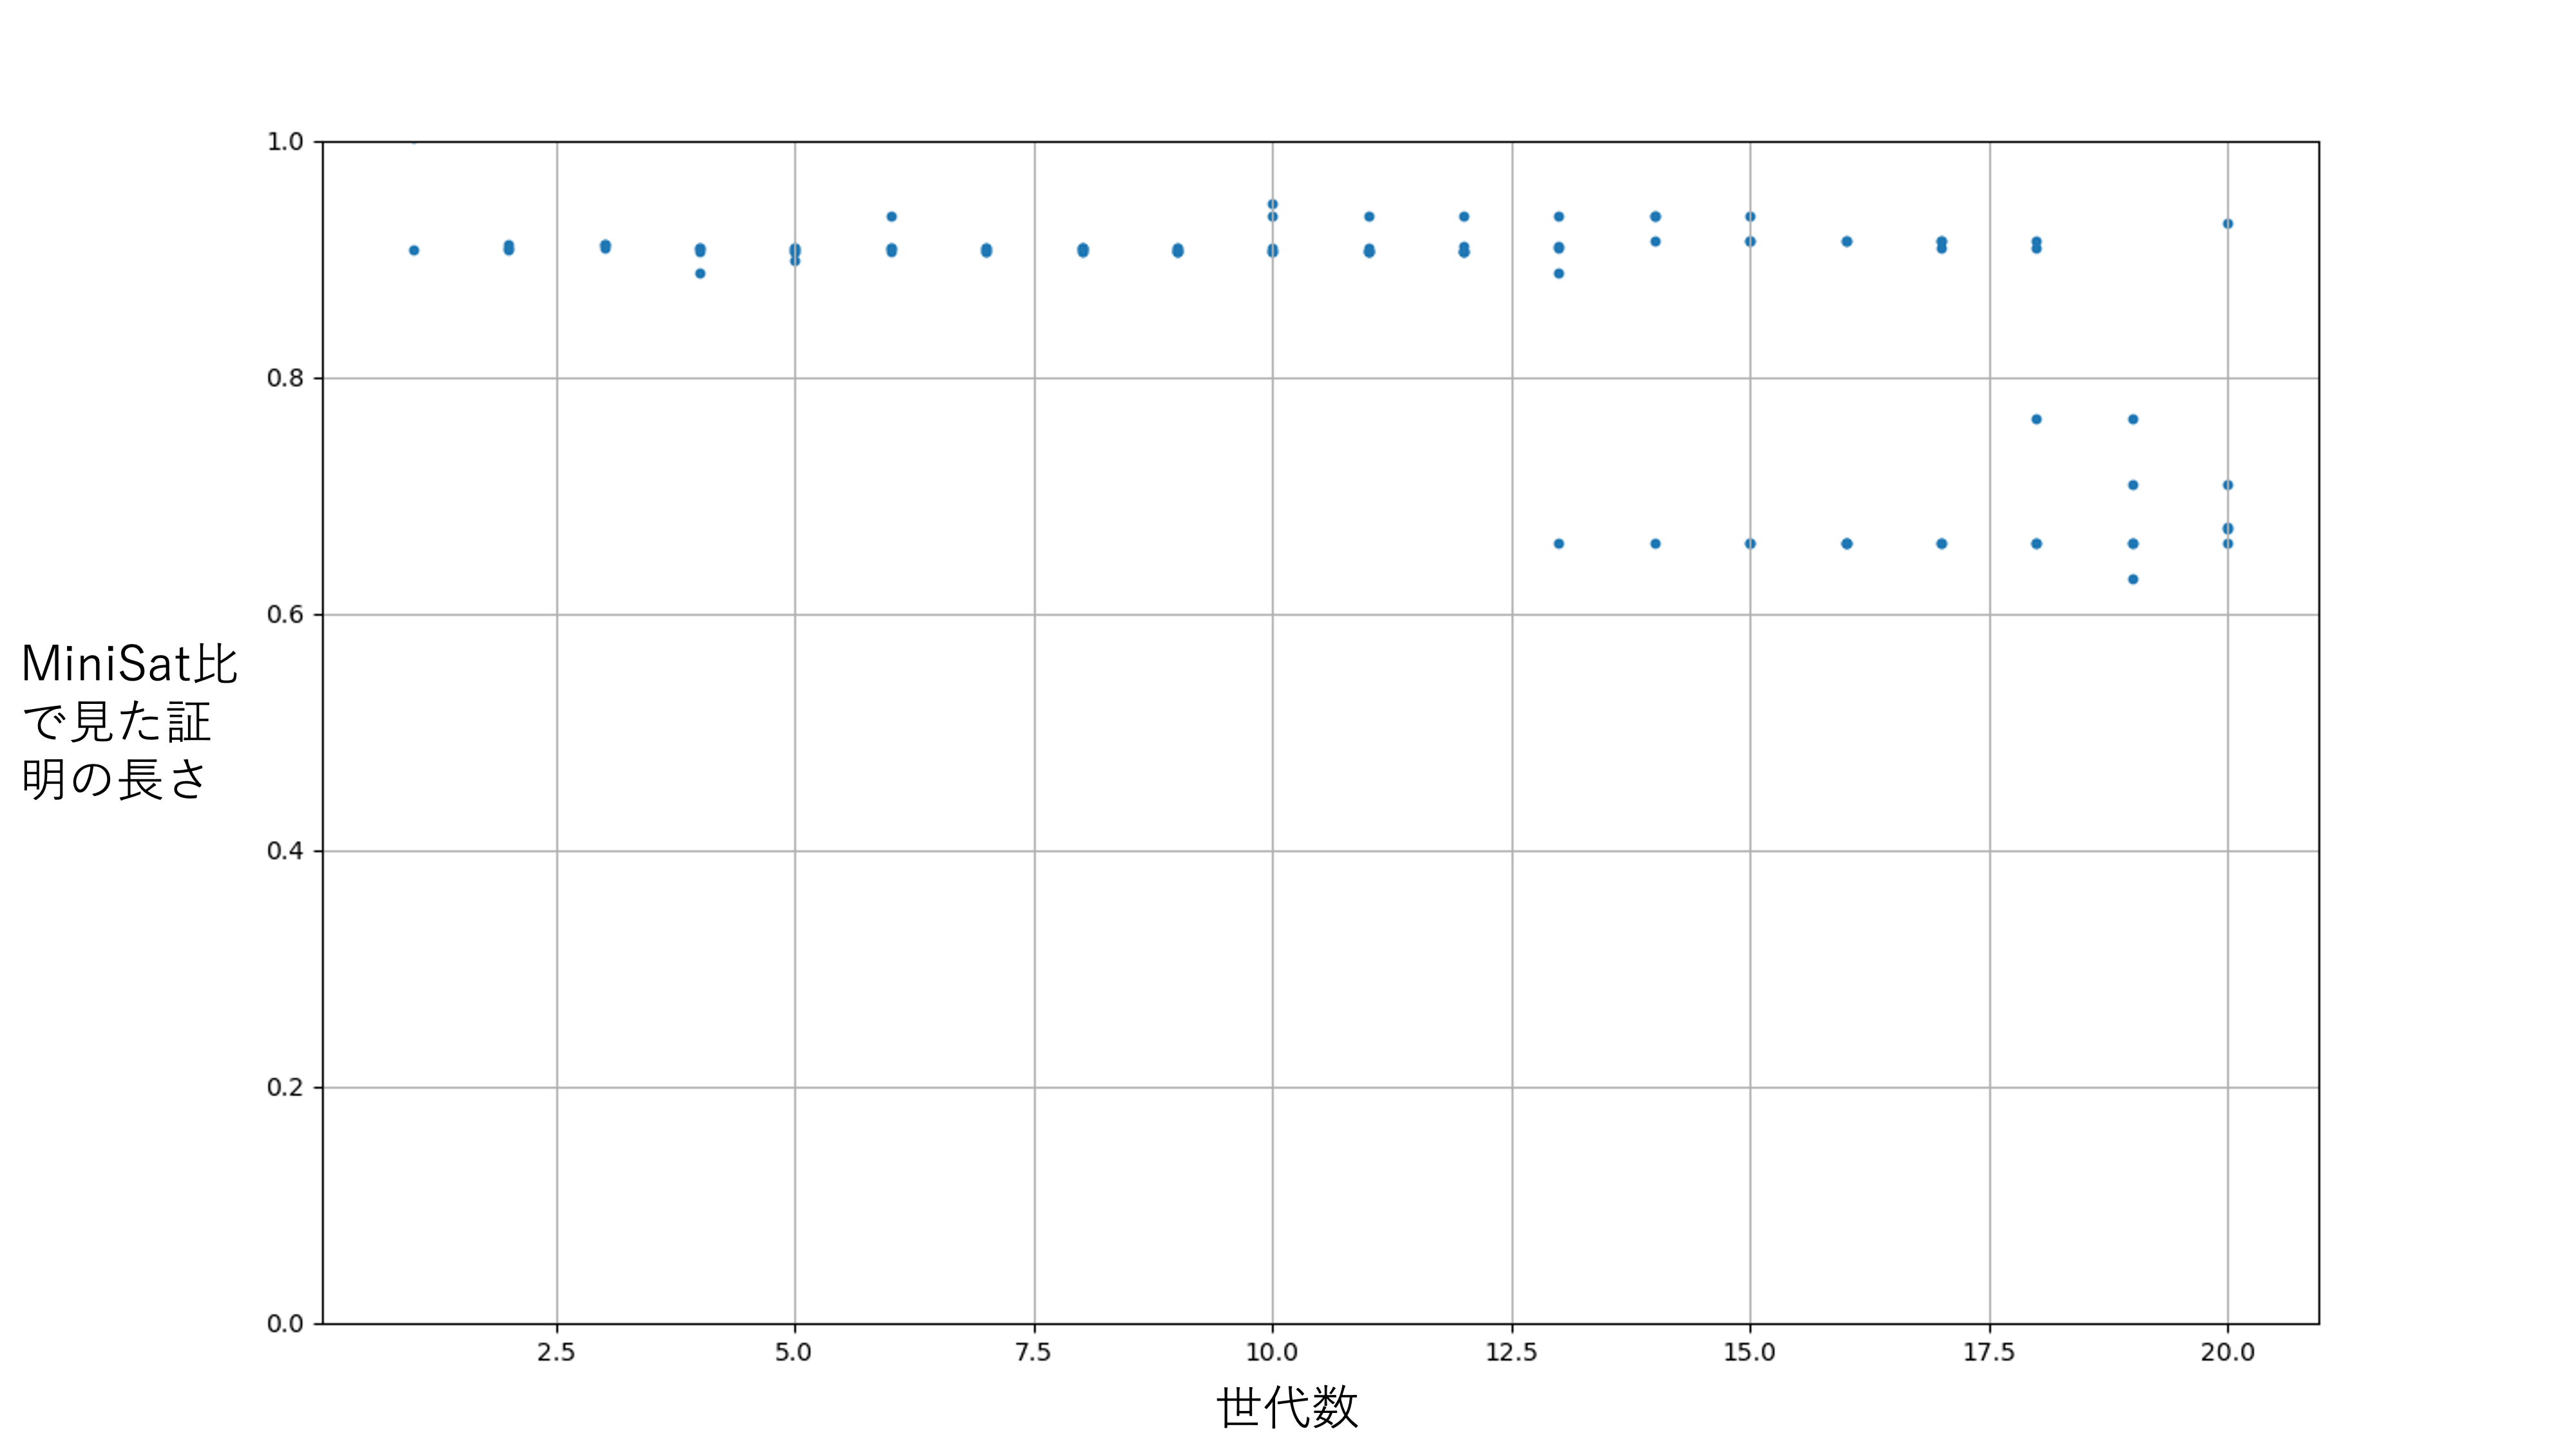
\includegraphics[width=10cm]{figures/Experiment1/1.png}
    \caption{初期パラメータにおける全染色体の証明長}
\end{figure}

2集団サイズ、試行回数を増やす

 ・サイズ20 * 世代25

 ・初期介入回数10 % 実験中

\begin{figure}[h]
    \centering
    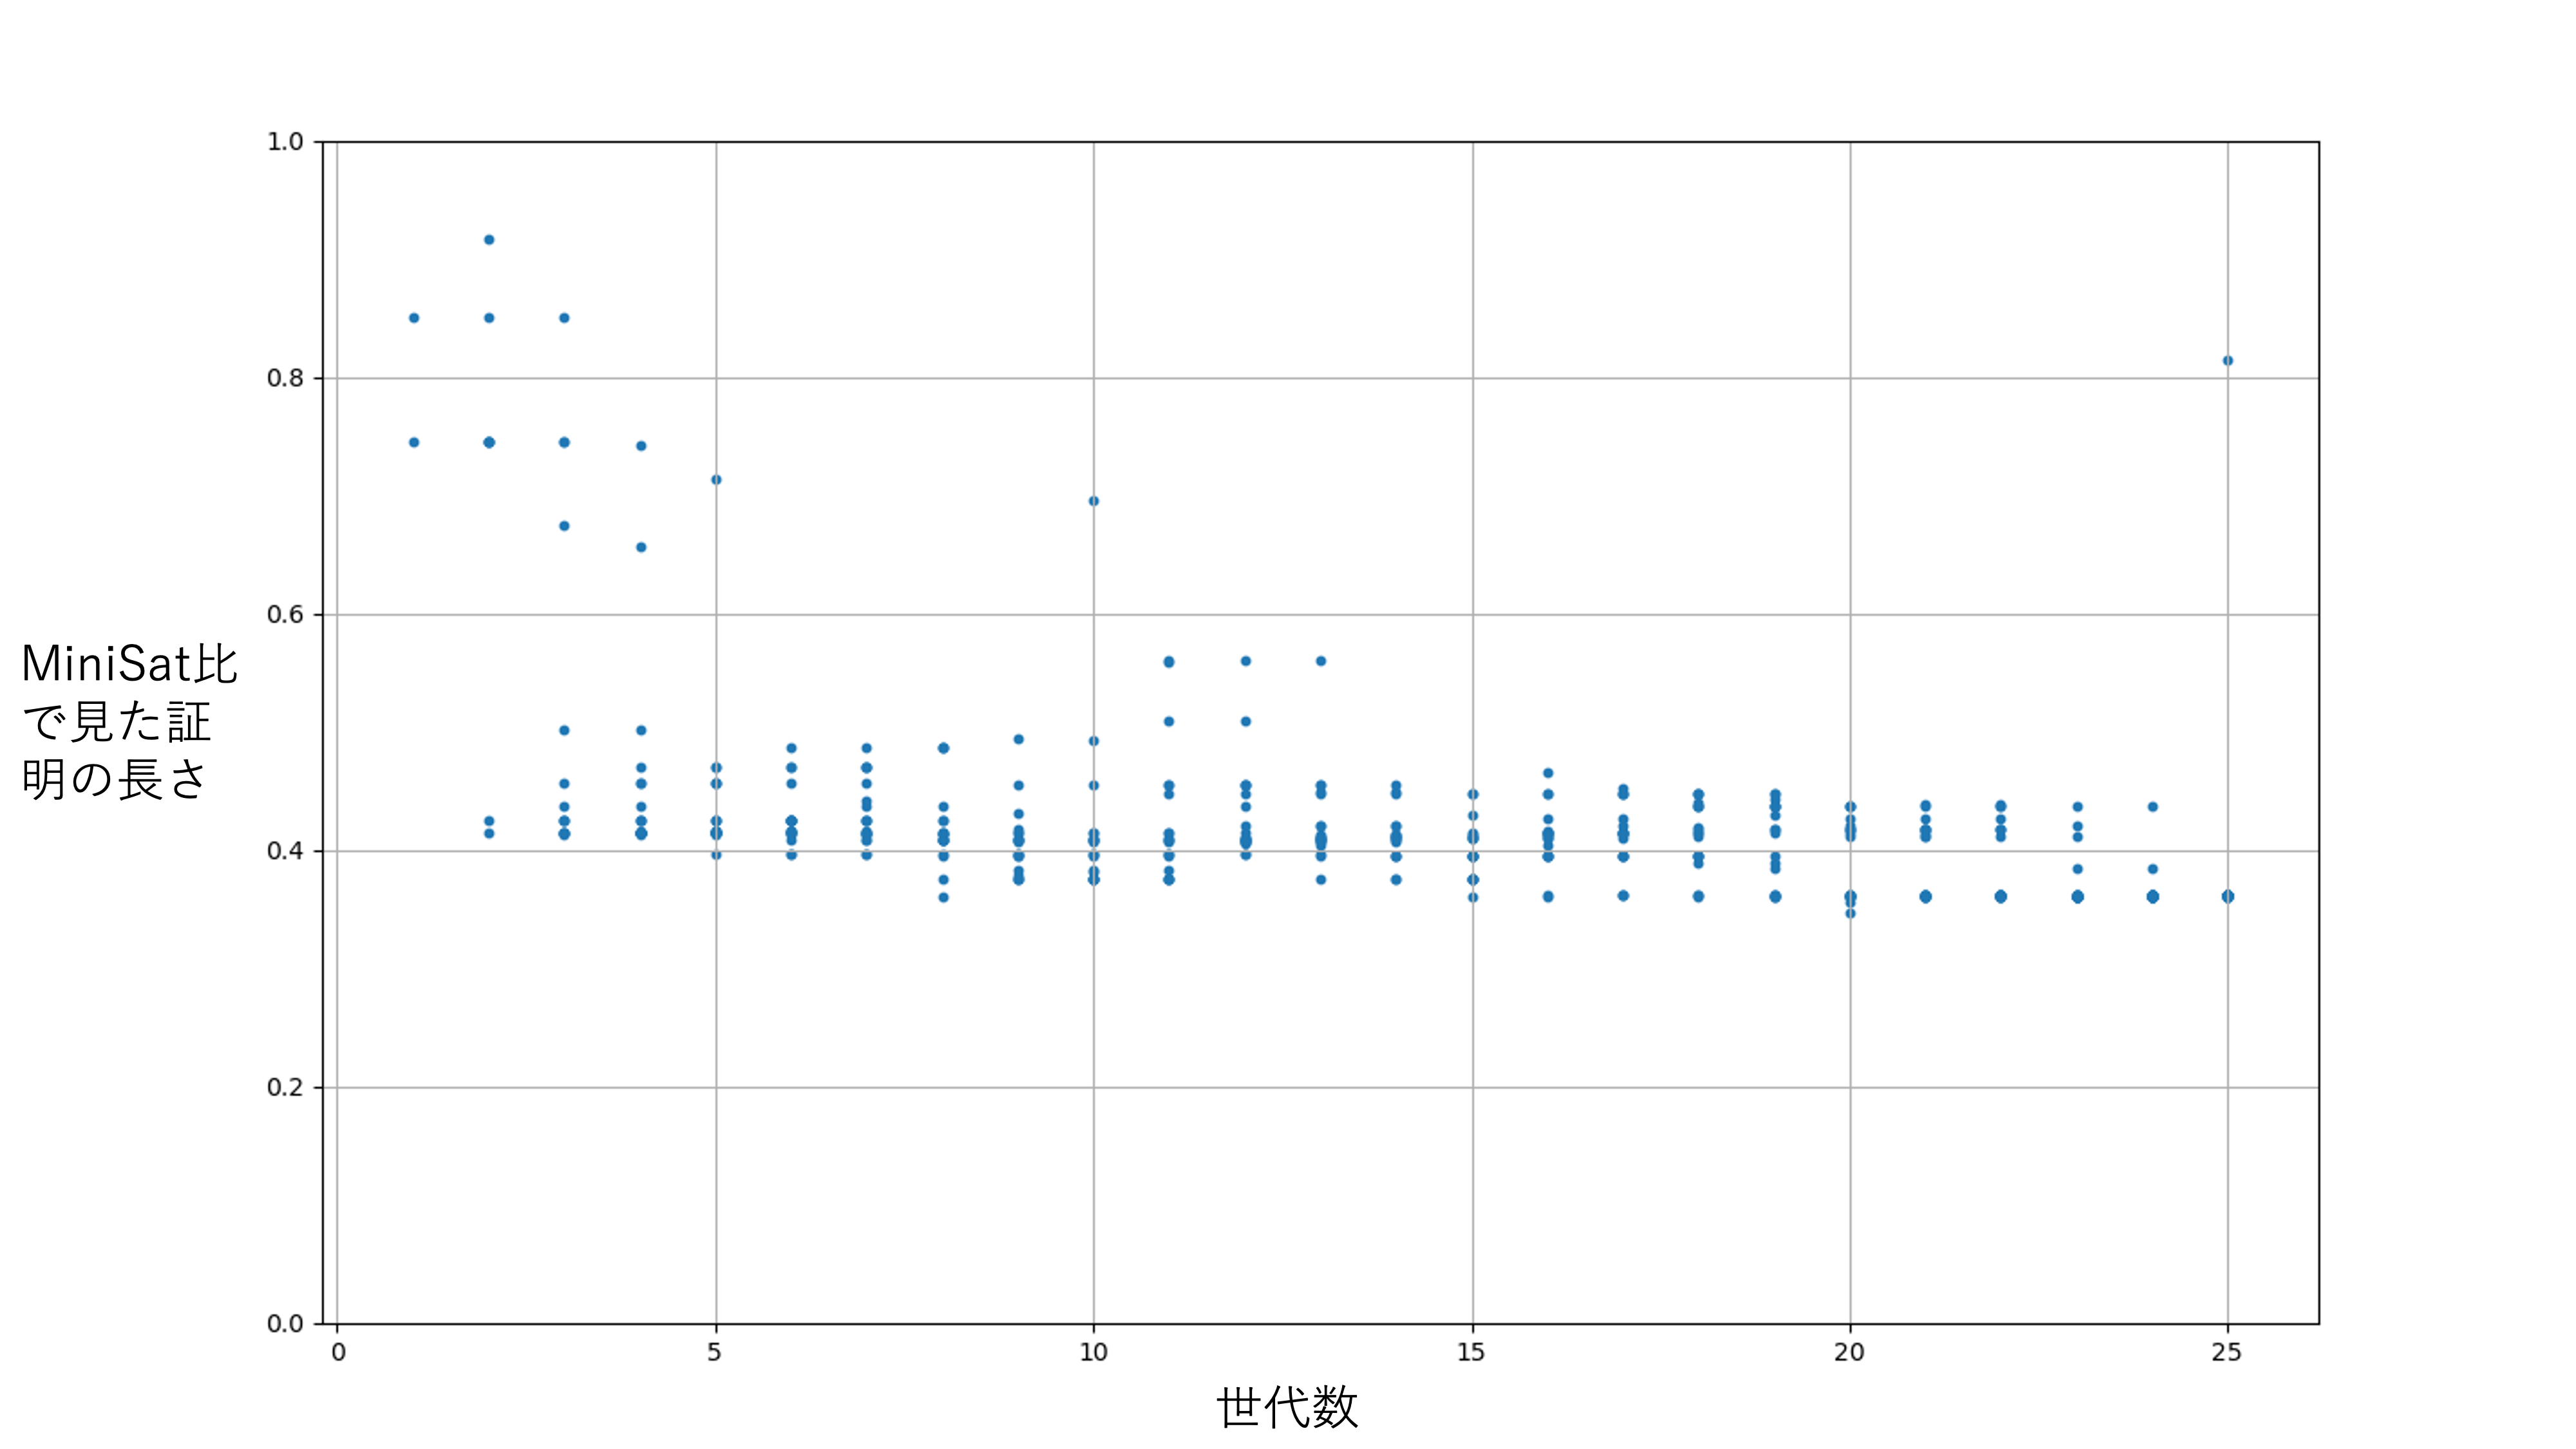
\includegraphics[width=10cm]{figures/Experiment1/2.png}
    \caption{集団サイズと世代を増加}
\end{figure}

3介入の回数をランダムに

 ・20 * 25

 ・初期介入回数ランダム

\begin{figure}[h]
    \centering
    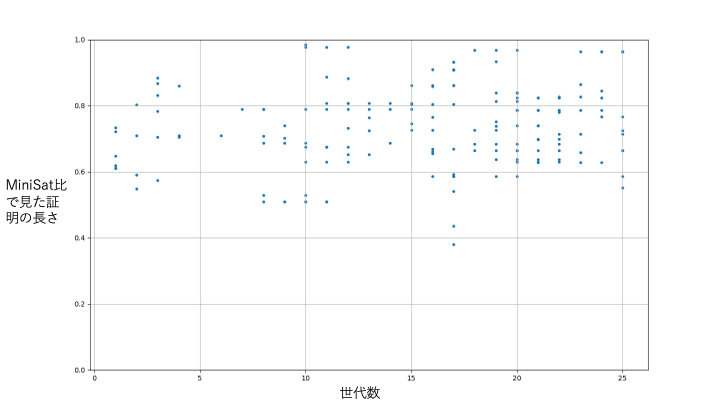
\includegraphics[width=10cm]{figures/Experiment1/3.png}
    \caption{初期の介入回数をランダムに}
\end{figure}

 ・多様性が増えた

 ・どの介入もなんか収束してそう

\begin{figure}[h]
    \centering
    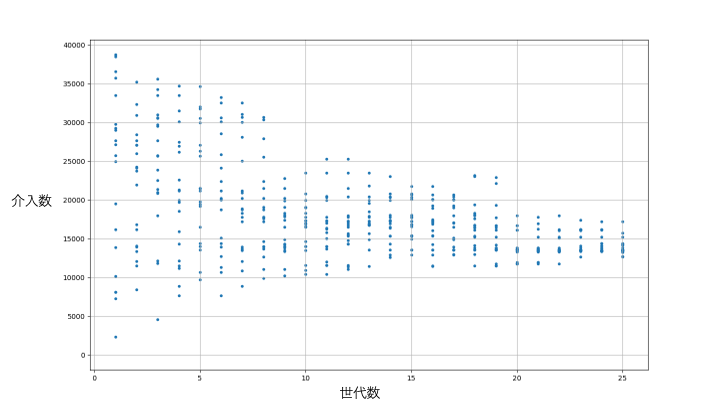
\includegraphics[width=10cm]{figures/Experiment1/3-1.png}
    \caption{介入回数の遷移}
\end{figure}

  ・初期の介入回数を10000以上20000以下に

\begin{figure}[h]
    \centering
    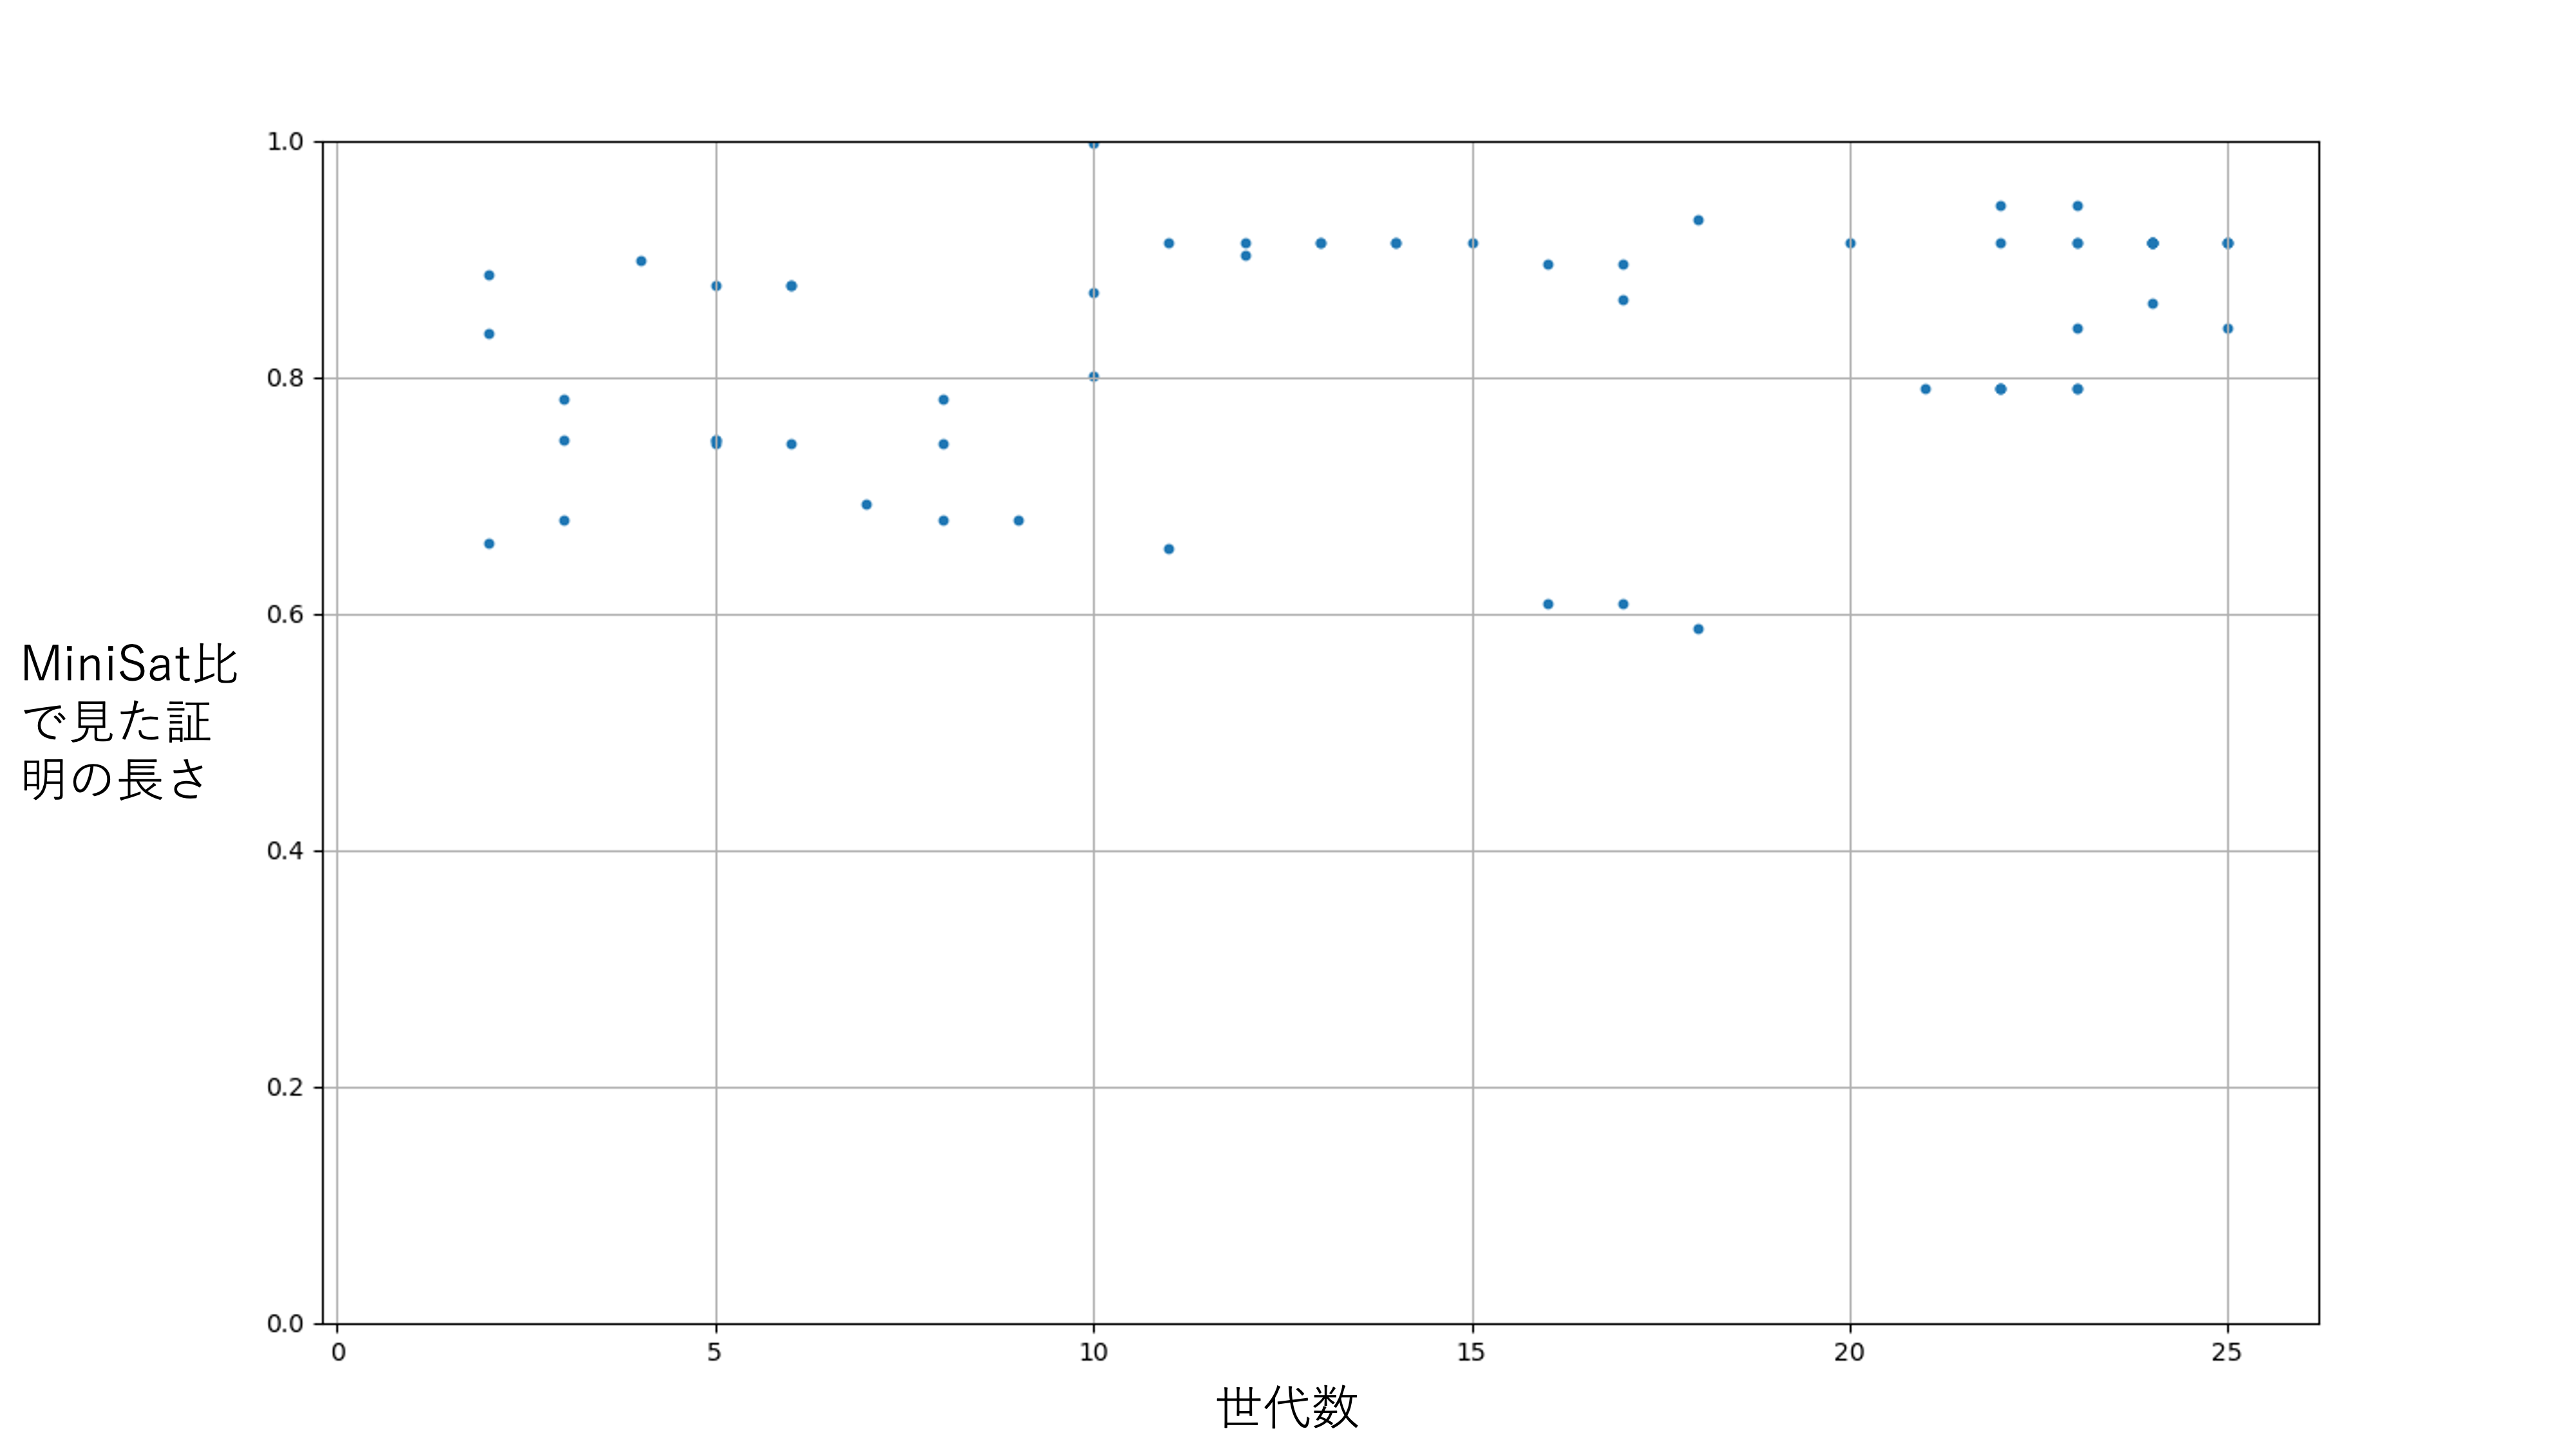
\includegraphics[width=10cm]{figures/Experiment1/3-2.png}
    \caption{介入回数を10000以上20000以下で始める}
\end{figure}

・介入をランダムにしてその状態での集団サイズと試行回数を調べた

4集団サイズと世代の変更

\begin{figure}[h]
    \centering
    \begin{minipage}{0.43\columnwidth}
        \centering
        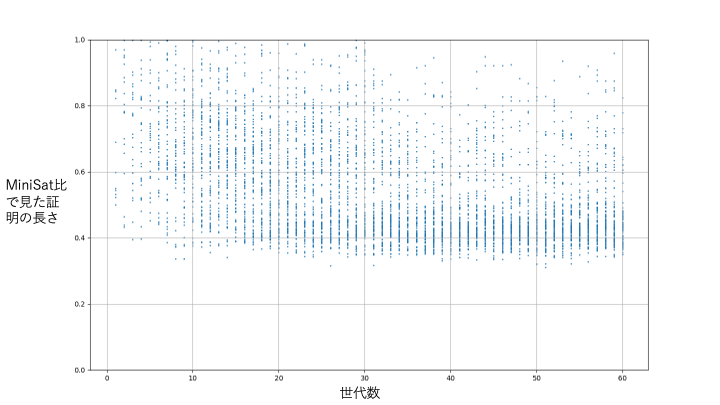
\includegraphics[width=\columnwidth]{figures/Experiment1/4-1.png}
        \caption{サンプルA}
        \label{fig:サンプルA}
    \end{minipage}
    \hspace{5mm}
    \begin{minipage}{0.43\columnwidth}
        \centering
        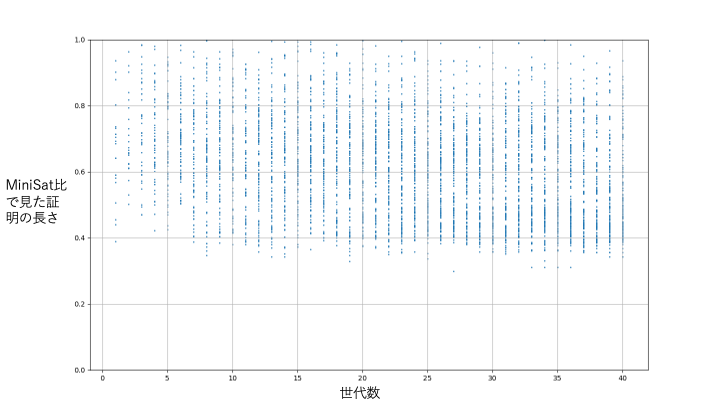
\includegraphics[width=\columnwidth]{figures/Experiment1/4-2.png}
        \caption{サンプルB}
        \label{fig:サンプルB}
    \end{minipage}
  
    \vspace{3mm}
    
    \begin{minipage}{0.43\columnwidth}
        \centering
        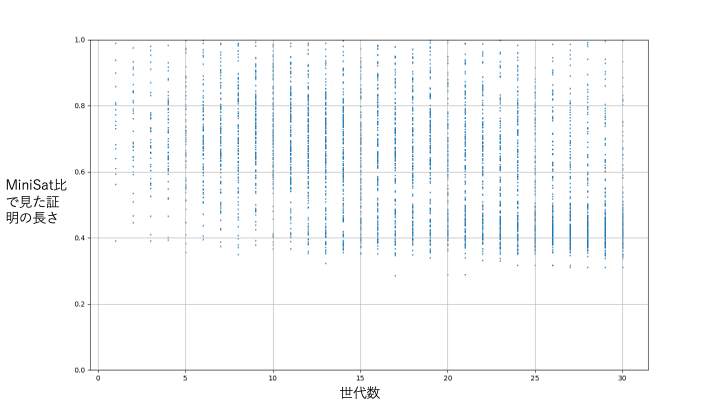
\includegraphics[width=\columnwidth]{figures/Experiment1/4-3.png}
        \caption{サンプルC}
        \label{fig:サンプルC}
    \end{minipage}
    \hspace{5mm}
    \begin{minipage}{0.43\columnwidth}
        \centering
        
\includegraphics[width=\columnwidth]{figures/white.png}
    \end{minipage}
\end{figure}

5突然変異の変更
\begin{figure}[h]
    \centering
    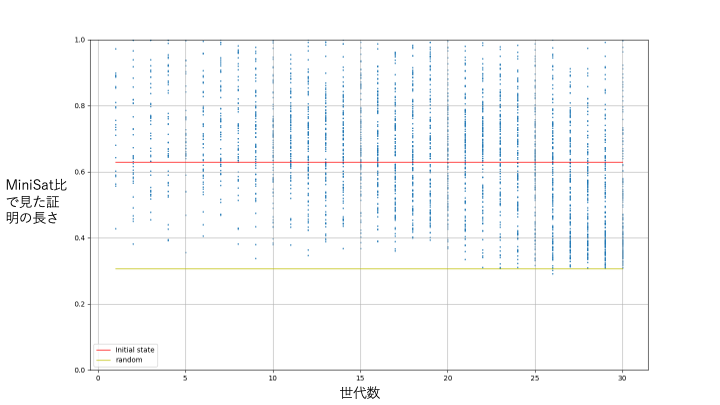
\includegraphics[width=10cm]{figures/Experiment1/5.png}
    \caption{突然変異の変更}
\end{figure}

6ランダムとの比較

7trim前の適応度の比較

\subsection{色々な問題に対して解く}%6ページ

・同じくらいの問題を解く

・長い問題を解く

・各問題のベストを見る

・空いている部分の問題を解く

・学習が続いている問題をを解く

\subsection{kissatとの比較}%4ページ

・kissatとの比較

\subsection{今後のために少し調べたこと}

・適応度を2乗に